\documentclass[pdf]{beamer}
%\usetheme{ENSTB}
\usetheme{Pittsburgh}
%\usetheme{Warsaw}

%\usepackage{time}       % date and time
\usepackage{graphicx}
\usepackage[T1]{fontenc}    % european characters
%\usepackage{courier}
\usepackage{amssymb,amsmath}  % use mathematical symbols
\usepackage{palatino}                  % use palatino as the default font
\setbeamercovered{transparent}

\begin{document}

% here you define the information that will be displayed in the title/cover page
\title[IPsec and IKEv2 for the Contiki OS]{IPsec and IKEv2 for the Contiki OS\\}
\subtitle{Secure communication and the Internet of Things}
\author[Vilhelm Jutvik]{Vilhelm Jutvik\\Uppsala University\\}

%\vspace*{0.5cm}    
%\includegraphics[height=0.5cm]{./figures/e-mail}

%\date{11th December 2006}

% this is used in the pdf information
\subject{IPsec and IKEv2 for the Contiki OS}

% here you build the title page
 \frame{
  \titlepage
 }

% outline
% \AtBeginSection[]
% {
%  \begin{frame}
%   \frametitle{Outline}
%   \small
%   \tableofcontents[currentsection,hideothersubsections]
%   \normalsize
%  \end{frame}
% }

\section{The case for the IoT}
\begin{frame}
   \frametitle{The case for IoT}
   The IoT will bring cheap and flexible communication to our everyday things
%   \pause Features
   %S: We've been tasked by the ACME corporation to create the ultimate home entertainment solution
%   \begin{itemize}
%      \pause \item Photo slideshow
%      \pause \item Play movies
%      \pause \item TiVo feature
%   \end{itemize}
\end{frame}


\section{Introduction}
\begin{frame}
   \frametitle{Problem statement}
   As the IoT will control and monitor sensors as well as machines in our surroundings, security is a natural concern. There is no consensus of how to deal with this issue.
%   \pause Features
   %S: We've been tasked by the ACME corporation to create the ultimate home entertainment solution
%   \begin{itemize}
%      \pause \item Photo slideshow
%      \pause \item Play movies
%      \pause \item TiVo feature
%   \end{itemize}
\end{frame}


\section{Introduction}
\begin{frame}
   \frametitle{Research question}
   
   IPsec and IKEv2 is one method of securing the Internet.
   \pause
   
   Question: Can IPsec and IKEv2 be implemented within the current hardware boundaries while still being interoperable with other Internet hosts?
 
%   What information do we need? \pause We need to understand how people does these things today.\\
   %S: To be more specific, we need the following information about each activity
%   \pause
\end{frame}

\begin{frame}
   \frametitle{Contiki}
   Contiki is an operating system designed for computers with severely constrained resources.
\end{frame}

\begin{frame}
   \frametitle{IPsec and IKEv2}
   Security in the IP (network) layer instead of in the application (like that of TLS).
\end{frame}


\begin{frame}
   \frametitle{Implementation}
   Using the method of experimental computer science, I implemented IPsec and IKEv2 on Contiki and evaluated it.

%   \includegraphics[scale=0.3]{bilder/office}
   %D: Shuffle
      
   %S: It's all about the context. This [office] is an official context, just look at their clothes, and this [family] is within the private sphere. We need to get close up to these families, we need to understand their habits, how their rules are created and what they love and hate. You don't divulge information like this to strangers.
\end{frame}


\begin{frame}
   \frametitle{Implementation: IPsec}
   IPsec was implemented as a part of Contiki's $\mu$IP stack.
\end{frame}

%\section{Interpretation}
\begin{frame}
   \frametitle{Implementation: IKEv2}
   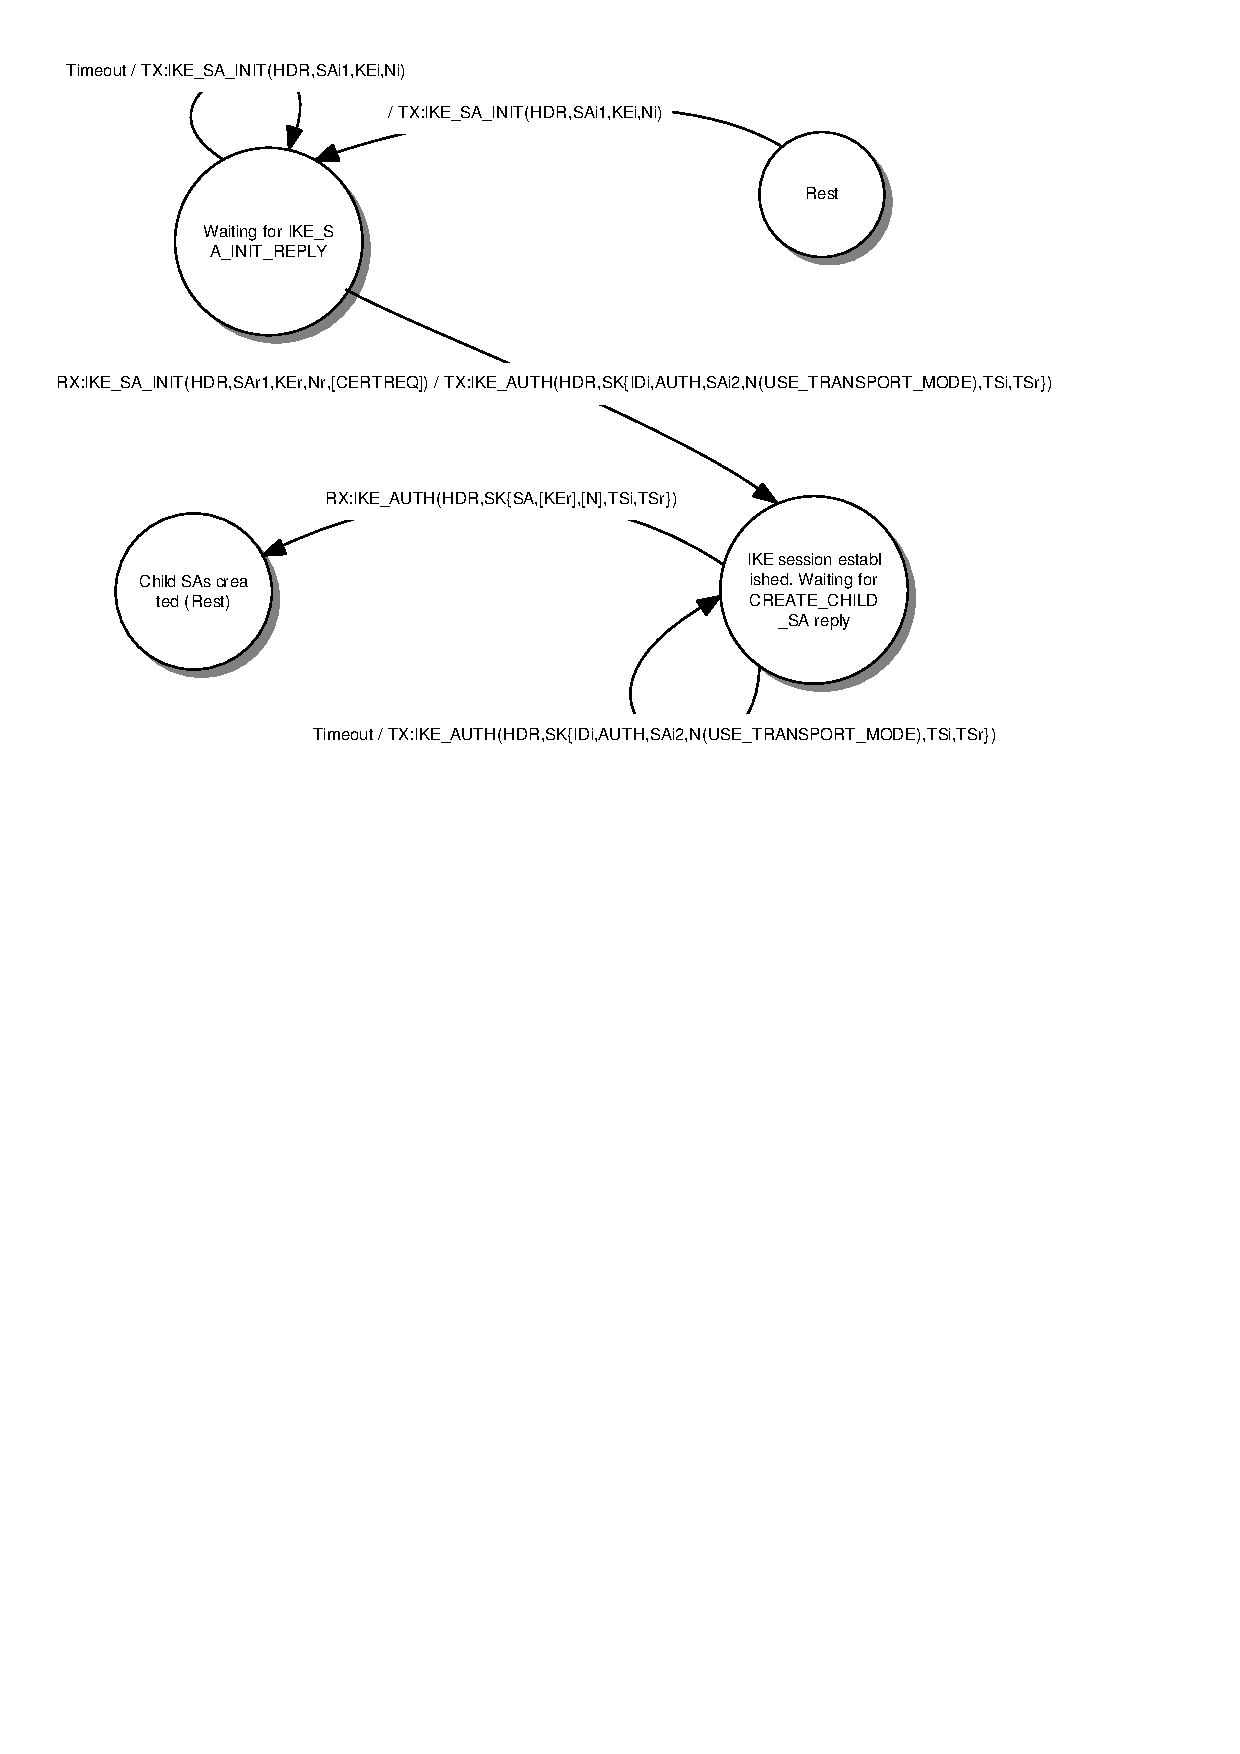
\includegraphics[scale=0.65]{bilder/initiator_mealy.png}
\end{frame}

\begin{frame}
   \frametitle{Supporting libraries}
   Porting TinyECC to Contiki: ContikiECC
\end{frame}

\begin{frame}
   \frametitle{Evaluation}
   ROM, RAM, heap and stack consumption was measured.
\end{frame}

\begin{frame}
   \frametitle{Conclusion}
   IPsec and IKEv2 can be used in Contiki on current hardware, but future platforms will make it practical. 
\end{frame}



\end{document}
   
   
   
   
   
   
   
   
   
   
   
   
% \section{Introduction}
% \begin{frame}
%    \frametitle{Overview}
%    \begin{itemize}
%       \item Recruit the Users
%       \pause
% 
%       \item Contextual Inquiry (interviews)
%       \pause
%       \item[$\Rightarrow$] Data about habits, attitudes etc
%       \pause
%       
%       \item Interpretation session
%       \pause
%       \item[$\Rightarrow$] Affinity diagrams (lots of post-it notes detailing people's issues/needs)
%       \pause
%       \item[$\Rightarrow$] Work models (that describes how people act)
%       \pause
%       
%       \item Consolidate models
%       \pause
%       
%       \item Do system design based on...
%       \pause
%       \item[$\Rightarrow$] The affinity diagrams
%       \pause
%       \item[$\Rightarrow$] The work models
%       \pause
%       
%       \item Iterating with prototypes
% 
%    \end{itemize}
% \end{frame}
%    
% 
% \begin{frame}
%     \frametitle{Who are the Users?}
%     \begin{itemize}
%         \item 
%         \item Services with high QoS requirements   gain momentum
%         \item Value lies in services
%         \pause
%         \item[$\Rightarrow$] Currently deployed networks need to adapt to these tendencies.
%      \item[$\Rightarrow$] The IP multimedia Subsystem is seen as a promising solution for fullfiling these needs.
%     \end{itemize}
% \end{frame}
% 
% %\part{Main Talk} % used for two reasons: structuring and decreasing outline granularity
% \begin{frame}
%     \frametitle{The IMS standards}
%      \begin{block}{3GPP}
%       initiated at the work on IMS (Release 5 - March 2003), focused on facilitated service development and deployment.
%       3GPP R7 underway.   
%      \end{block}
%      \pause
%      \begin{block}{ETSI TISPAN}
%         Extended IMS focus for network convergence purposes (Access agnostic) in the scope of the work on Next Generation Networks (NGN).
%         First release available. Second release underway.
%      \end{block}
%      \pause
%      \begin{block}{IETF}
%         In order to facilitate interoperability IMS specifies the use of open Internet protocols standardized at IETF.
%      \end{block}
% \end{frame}
% 
% 
% \section{Motivation for the use of IMS}
%     \subsection{Basic principles}
%     \begin{frame}
%         \frametitle{Easier network management}
%         \begin{itemize}
%             \item Separated control and bearer functions
%             \item All IP overlay service delivery on top of a packet switched architecture
%             \item Migration of Circuit Switched services to Packet Switched domain
%             \pause
%             \item[$\Rightarrow$] Network management savings
%         \end{itemize}
%     \end{frame} 
%    
% % \textsubrightarrow 
%    
%     \begin{frame}
%         \frametitle{End-to-end architecture}
%         \begin{itemize}
%             \item Service delivery independent of the access technology
%             \item Use of open Internet protocols
%             \item End-to-end QoS management (support for real-time services)
%             \pause
%             \item[$\Rightarrow $] Inherent contradiction: IMS relies on IP technologies allowing free communications but aims at controlling IP service delivery.
%         \end{itemize}
%     \end{frame}
